% Usage: knitr slide


\chapter{Challenges of Analyzing High-Dimensional Data}\alabel{chap:hdata}
\quoteit{
\textbf{Biomarker Uncertainty Principle}:\\
 A molecular signature can be either parsimonious or predictive, but
 not both.}{FE Harrell, 2009}

\quoteit{We have more data than ever, more good data than ever, a
  lower proportion of data that are good, a lack of strategic thinking
  about what data are needed to answer questions of interest,
  sub-optimal analysis of data, and an occasional tendency to do
  research that should not be done.}{FE Harrell, 2015}
  
\section{Background}
High-dimensional data are of at least three major types:
\bi
\item Data collected on hundreds of thousands or millions of subjects
  with a diverse array of variables
\item Time series of biologic signals collected every few milliseconds
\item Extremely large data arrays where almost all the variables are
  of one type (the main topic here)
\ei
The last data class includes such areas as
\bi
\item functional imaging
\item gene microarray
\item SNPs for genome-wide association studies
\item RNA seq
\item exome sequencing
\item mass spectrometry
\ei

The research yield of analysis of such data has been disappointing to
date, for many reasons such as:
\bi
\item Biology is complex
\item Use of non-reproducible research methodology
\item Use of unproven statistical methods
\item Multiple comparison problems and double dipping\footnote{Double
    dipping refers to using the same data to test a hypothesis that
    was formulated from a confession from the tortured dataset.}
\item Failure to demonstrate value of information over and above the
  information provided by routine clinical variables, blood chemistry,
  and other standard medical tests
\item Inadequate sample size for the complexity of the analytic task
\item Overstatement of results due to searching for ``winning''
  markers without understanding bias, regression to the mean
  (Section~\ref{sec:change-rttm}), and overfitting
\ei

Regarding double dipping/multiplicity a beautiful example is the dead
salmon fMRI study by Bennett~\emph{et al.} in which the standard
method of analyzing fMRI data by voxels was shown to find brain
activation regions even in the dead brain (see
\url{http://prefrontal.org/files/posters/Bennett-Salmon-2009.pdf}).

\centerline{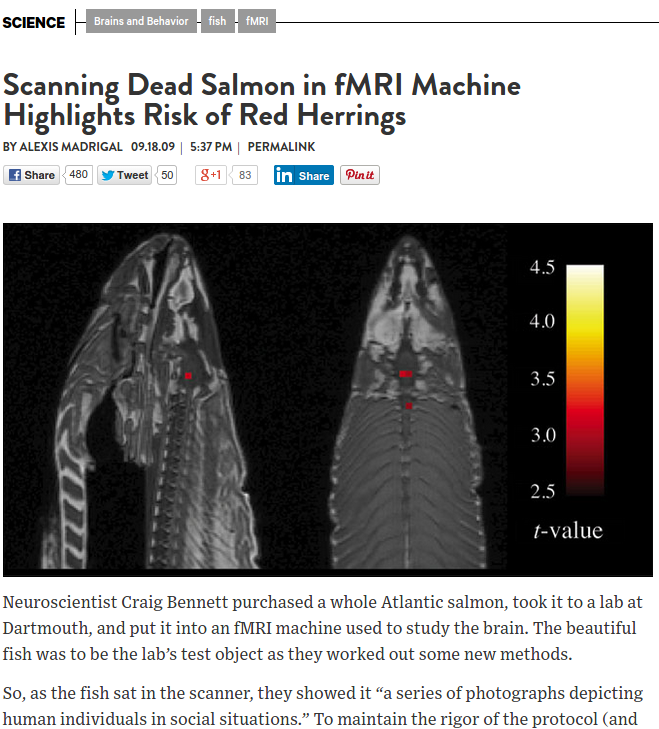
\includegraphics[width=.65\textheight]{deadsalmon.png}}

\emph{Wired}, 2009-09-18.

Unfortunately, a large number of papers in genomics and imaging
research have pretended that feature selection has no randomness, and
have validated predictions in the same dataset used to find the signals,
without informing the bootstrap or cross-validation procedure about
the data mining used to derive the model so that the resampling
procedure could repeat all feature selection steps afresh for each
resample~\cite{amb02sel}.  Only by re-running all data analysis steps
that utilized $Y$ for each resample can an unbiased estimate of future
model performance be obtained.

\section{Global Analytic Approaches}
Let $X_{1}, X_{2}, \ldots, X_{p}$ denote an array of candidate features (gene expressions, SNPs, brain activation, etc.) and $Y$ the response, diagnosis, or patient outcome being predicted.

\subsection{One-at-a-Time Feature Screening}
OaaT feature screening involves choosing a measure of association such as Pearson's $\chi^2$ statistic\footnote{Oddly, many practitioners of OaaT choose the more conservative and much slower to compute Fisher's exact test.}, computing all $p$ association measures against $Y$, and choosing those $X$ features whose association measure exceeds a threshold.   
This is by far the most popular approach to feature discovery (and often to prediction, unfortunately) in genomics and functional imaging.  It is demonstrably the worst approach in terms of the reliability of the ``winning'' and ``losing'' feature selection and because it results in poor predictive ability.  The problems are due to multiple comparison problems, bias, typically high false negative rates, and to the fact that most features ``travel in packs'', i.e., act in networks rather than individually.  As if OaaT could not get any worse, many practitioners create ``risk scores'' by simply adding together individual regression coefficients computed from individual ``winning' $X$ features without regard to the correlation structure of the $X$s.  This gives far too much weight to the selected $X$s that are co-linear with each other.

There is a false belief that preventing a high false discovery rate solves the problems of OaaT.  Most researchers fail to consider, among other things, the high false negative rate caused by their design and sample size.

OaaT results in highly overestimated effect sizes for winners, due to
double dipping.

\subsubsection{Multiplicity Corrections}
In the belief that false positive discoveries are less desirable than
missed discoveries, researchers employ multiplicity corrections to
$P$-values arising from testing a large number of associations with
$Y$.  The most conservative approach uses the addition or Bonferroni
inequality to control the \emph{family-wise error risk} which is the
probability of getting \emph{any} false positive association when the global
null hypothesis that there are no true associations with $Y$ holds.
This can be carried out by testing the $p$ associations against
$\frac{\alpha}{p}$ where $\alpha=0.05$ for example.  A less
conservative approach uses the \emph{false discovery rate} (FDR),
better labeled the \emph{false discovery risk} or \emph{false
  discovery probability}.  Here one controls the fraction of false
positive associations.  For example one sets the critical value for
association statistics to a less severe threshold than dictated by
Bonferroni's inequality, by allowing $\frac{1}{10}^{\mathrm th}$ of
the claimed associations (those with the smallest $P$-values) to be
false positives.

It is an irony that the attempt to control for multiplicity has led
not only to missed discoveries and abandonment of whole research areas
but has resulted in increased bias in the ``discovered'' features'
effect estimates.  When using stepwise regression, the bias in
regression coeffients comes not from multiplicity problems arising
when experimentwise $\alpha=0.05$ is used throughout but from using an
$\alpha$ cutoff $< \frac{1}{2}$ for selecting variables.  By selecting
variables on the basis of small $P$-values, many of the selected
variables were selected because their effects were overestimated, then
regression to the mean sets in.

\subsection{Forward Stepwise Variable Selection}
Forward stepwise variable selection that does an initial
screening of all the features, adds the most significant one, then
attempts to add the next most significant feature, after adjusting
for the first one, and so on.  This approach is unreliable.  It is
only better than OaaT in two ways: (1) a feature that did not meet the
threshold for the association with $Y$ without adjusting for other
features may become stronger after the selection of other features at
earlier steps, and (2) the resulting risk score accounts for
co-linearities of selected features.  On the downside, co-linearities
make feature selection almost randomly choose features from correlated
sets of $X$s, and tiny changes in the dataset will result in different
selected features. 

\subsection{Ranking and Selection}
Feature discovery is really a ranking and selection problem.  But ranking and selection methods are almost never used.  An example bootstrap analysis on simulated data is presented later.  This involves sampling with replacement from the combined $(X, Y)$ dataset and recomputing for each bootstrap repetition the $p$ association measures for the $p$ candidate $X$s.  The $p$ association measures are ranked.  The ranking of each feature across bootstrap resamples is tracked, and a 0.95 confidence interval for the rank is derived by computing the 0.025 and 0.975 quantiles of the estimated ranks.

This approach puts OaaT in an honest context that fully admits the true difficulty of the task, including the high cost of the false negative rate (low power).  Suppose that features are ranked so that a low ranking means weak estimated association and a high ranking means strong association.  If one were to consider features to have ``passed the screen'' if their lower 0.95 confidence limit for their rank exceeds a threshold, and only dismisses features from further consideration if the upper confidence limit for their rank falls below a threshold, there would correctly be a large middle ground where features are not declared either winners or losers, and the researcher would be able to only make conclusions that are supported by the data.  Readers of the class \emph{Absence of Evidence} paper~\cite{alt95abs} will recognize that this ranking approach solves the problem.

An example of bootstrap confidence intervals where multivariable modeling was used rather than OaaT association measures is in the course notes for \emph{Regression Modeling Strategies}, Section~5.4.  An example where the bootstrap is used in the context of OaaT is below.

\subsection{Joint modeling of All Features Simultaneously using Shrinkage}
This approach uses multivariable regression models along with penalized maximum likelihood estimation, random effects / hierarchical modeling, or skeptical Bayesian prior distributions for adjusted effects of all $p$ $X$ features simultaneously.  Feature effects (e.g., log odds ratios) are discounted so as to prevent overfitting/over-interpretation and to allow these effects to be trusted out of context.  The result is a high-dimensional regression model that is likely to provide well-calibrated absolute risk estimates and near-optimum predictive ability.  Some of the penalization methods used are
\be
\item lasso: a penalty on the absolute value of regression coefficient that highly favors zero as an estimate.  This results in a large number of estimated coefficients being exactly zero, i.e., results in feature selection.  The resulting parsimony may be illusory: bootstrap repetition may expose the list of ``selected'' features to be highly unstable.
\item ridge regression (penalty function that is quadratic in the regression coefficients): does not result in a parsimoneous model but is likely to have the highest predictive value
\item elastic net: a combination of lasso and quadratic penalty that has some parsimony but has better predictive ability than the lasso.  The difficulty is simultaneously choosing two penalty parameters (one for absolute value of $\beta$s, one for their sum of squares).
\ee

\subsection{Random Forest}
This is an approach that solves some of the incredible instability and low predictive power of individual regression trees.  The basic idea of random forest is that one fits a regression tree using recursive partitioning (CART) on multiple random samples of \textbf{candidate features}.  Multiple trees are combined.  The result is no longer a tree; it is an uninterpretable black box.  But in a way it automatically incorporates shrinkage and is often competitive with other methods in predictive ability.

There is evidence that minimal-assumption methods such as random
forests are ``data hungry'', requiring as many as 200 events per
candidate variable for their apparent predictive discrimination to not
decline when evaluated in a new sample~\cite{plo14mod}.

\subsection{Data Reduction Followed by Traditional Regression Modeling}
This approach uses techniques such as principle component analysis (PCA) whereby a large number of candidate $X$s are reduced to a few summary scores.  PCA is based on additively combining features so as to maximize the variation of the whole set of features that is explained by the summary score.  A small number of PCA scores are then put into an ordinary regression model (e.g., binary logistic model) to predict $Y$.  The result is sometimes satisfactory though no easier to interpret than shrinkage methods.

\subsection{Model Approximation}
Also called \emph{pre-conditioning}, this method is general-purpose and promising~\cite{pau08pre,she04inf,amb02sim}.  One takes a well-performing black box (e.g., random forest or full penalized regression with $p$ features) that generates predicted responses $\hat{Y}$ and incorporates the right amount of shrinkage to make the predictions well-calibrated.  Then try to find a smaller set of $X$s that can represent $\hat{Y}$ with high accuracy (e.g., $R^{2} \geq 0.9$).  Forward stepwise variable selection may be used for this purpose\footnote{Here one is developing a mechanistic prediction where the true $R^{2}$ is 1.0.}. This sub-model is an approximation to the ``gold-standard'' full black box.  The ability to find a well-performing approximation is a test of whether the predictive signal is parsimoneous.  If one requires 500 $X$s to achieve an $R^{2} \geq 0.9$ in predicting the gold-standard predictions $\hat{Y}$, then it is not possible to be parsimoneous and predictive.

A major advantage of model approximation is that if the original complex model was well calibrated by using appropriate shrinkage, the smaller approximate model inherits that shrinkage.

\subsection{Incorporating Biology into High-Dimensional Regression Models}
This approach is likely to result in the most trustworthy discoveries as well as the best predictive accuracy, if existing biological knowledge is adequate for specification of model structure.  This is a structured shrinkage method where pathway (e.g., gene pathway) information is inserted directly in the model.  One may encode multiple paths into a simultaneous regression model such that genes are ``connected'' to other genes in the same pathway.  This allows an
  entire path to be emphasized or de-emphasized.

\section{Simulated Examples}
Monte Carlo simulation, when done in a realistic fashion, has the
great advantage that one knows the truth, i.e., the true model and
values of model parameters from which the artificial population was
simulated.  Then any derived model or estimates can be compared to the
known truth.  Also with simulation, one can easily change the sample
size being simulated so that the effect of sample size can be studied
and an adequate sample size that leads to reliable results can be
computed.  One can also easily change the dimensionality of the features.

\subsection{Simulation To Understand Needed Sample Sizes}
One of the most common association measures used in genomic studies is
the odds ratio.  As shown in Section~\ref{sec:prop-rem} and
Figure~\ref{fig:prop-mmeor} , the odds
ratio (OR) is very difficult to estimate when the outcome is rare or when a
binary predictive feature has a prevalence far from $\frac{1}{2}$.
That is for the case when only a single pre-specified is estimated.
When screening multiple features for interesting associations, one is
effectively estimating a large number of ORs, and in order to make
correct decisions about which features are promising and which aren't,
one must be able to control the margins of error of the entire set of
OR estimates.

In the following simulation consider varying sample size $n$ and
number of candidate features $p$.  We simulate $p$ binary features
with known true ORs against the diagnosis or outcome $Y$.  The
true unknown ORs are assumed to have a normal$(\mu=0,\sigma=0.25)$
distribution.  We want to judge the ability to jointly estimate $p$
associations and to rank order features by observed associations.  The analysis
that is simulated does not examine multiple $X$s simultaneously, so we save time
by simulating just the total numbers of zeros and ones for each $X$, given $Y$.

\begin{Schunk}
\begin{Sinput}
# For a vector of n binary outcomes y, simulates p binary features
# x that have a p-vector of fixed prevalences | y=0 of prev and are connected
# to y by a p-vector of true population odds ratios ors.
# Estimates the p odds ratios against the simulated outcomes and
# returns a data frame summarizing the information
#
# Note: the odds ratio for x predicting y is the same as the odds ratio
# for y predicting x.  y is simulated first so that all features will
# be analyzed against the same outcomes

sim <- function(y, prev, or) {
  n <- length(y)
  p <- length(prev)
  if(p != length(or)) stop('prev and or must have the same length')

  # prev = Pr(x=1 | y=0); let the odds for this be oprev = prev / (1-prev)
  # or = odds(x=1 | y=1) / oprev
  # Pr(x=1 | y=1) = oprev / ((1 / or) + oprev)

  oprev <- prev / (1 - prev)
  p1 <- oprev / ((1 / or) + oprev)
  n0 <- sum(y == 0)
  n1 <- sum(y == 1)
  # For n0 observations sample x so that Pr(x=0 | y=0) = prev
  nxy0 <- rbinom(p, size=n0, prob=prev)
  nxy1 <- rbinom(p, size=n1, prob=p1)

  # Compute p sample odds ratios
  sor <- (n0 - nxy0) * nxy1 / (nxy0 * (n1 - nxy1))
  g <- function(x) ifelse(x >= 1, x, 1 / x)
  r1 <- rank(sor)[which.max(or) ] / p
  r2 <- rank(or) [which.max(sor)] / p
  data.frame(prev, or, nx=nxy0 / n0, obsprev0=(nxy0 + nxy1) / n,
             obsprev=nxy1 / (nxy0 + nxy1), obsor=sor, n=n,
             N       =paste('n', n, sep=':'),
             Features=paste('Features', p, sep=':'),
             mmoe    =quantile(g(sor / or), 0.90, na.rm=TRUE),
             obsranktrue=r1, truerankobs=r2,
             rho=cor(sor, or, method='spearman', use='pair'))
}
\end{Sinput}
\end{Schunk}

\begin{Schunk}
\begin{Sinput}
U <- NULL
set.seed(1)
for(n in c(50, 100, 250, 500, 1000, 2000)) {
  for(p in c(10, 50, 500, 1000, 2000)) {
    for(yprev in c(.1, .3)) {
      y <- rbinom(n, 1, yprev)
      prev <- runif(p, .05, .5)
      or <- exp(rnorm(p, 0, .25))
      u <- cbind(sim(y, prev, or),
                 Yprev=paste('Prevalence of Outcome', yprev, sep=':'))
      U <- rbind(U, u)
    }
  }
}
\end{Sinput}
\end{Schunk}

In the plots below red lines show the line of identity.

\begin{Schunk}
\begin{Sinput}
require(ggplot2)
pl <- function(yprev) {
  br <- c(.01, .1, .5, 1, 2.5, 5, 25, 100)
  ggplot(subset(U, Yprev=yprev),
         aes(x=or, y=obsor)) + geom_point() + facet_grid(Features ~ N) +
         ggtitle(paste('Prevalence of Outcome', yprev, sep=':')) +
         xlab('True ORs') + ylab('Estimated ORs') +
         scale_x_log10(breaks=br) + scale_y_log10(breaks=br) +
         theme(axis.text.x = element_text(size = rel(0.8), angle=-45,
                                    hjust=0, vjust=1)) +
         geom_abline(col='red')
}
pl(0.1)
\end{Sinput}


\centerline{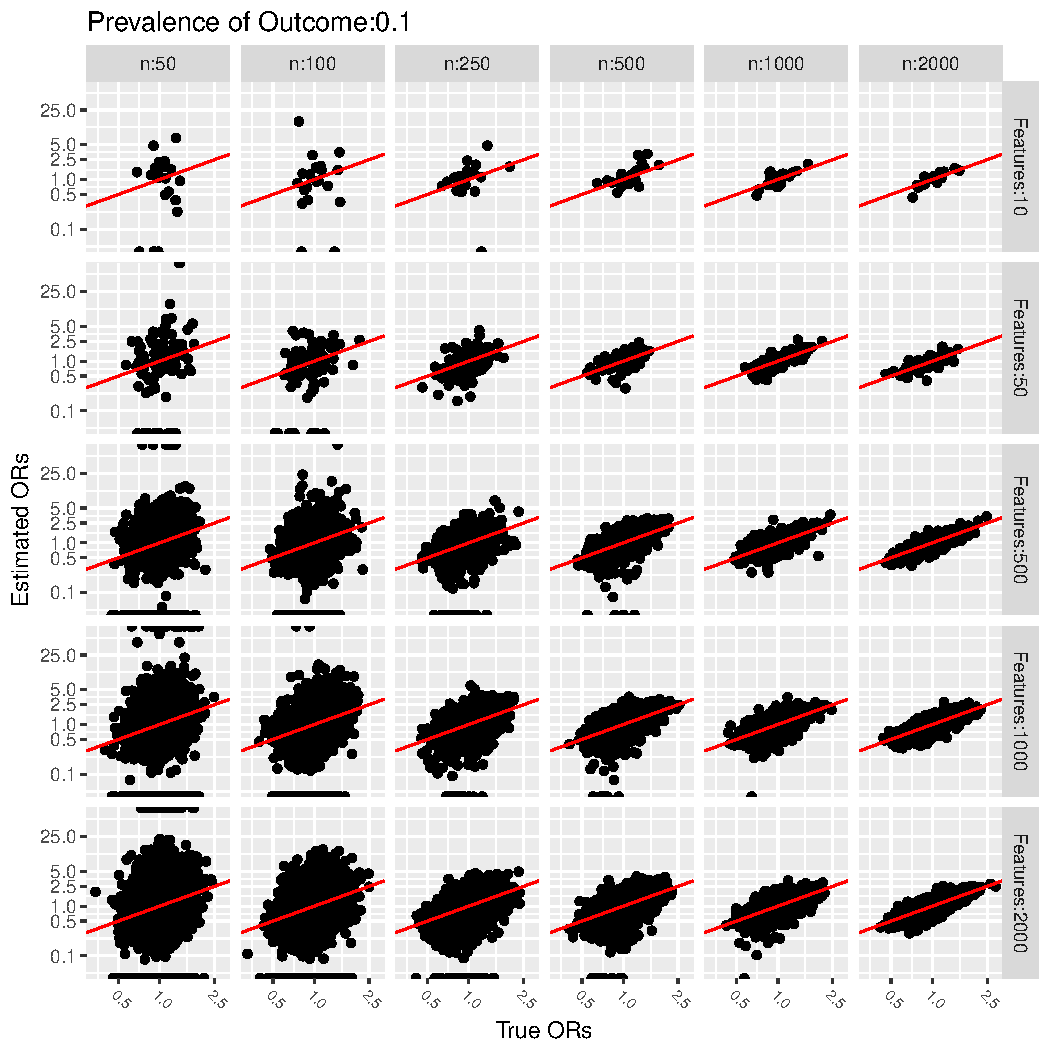
\includegraphics[width=\maxwidth]{hdata-simor-plot-1} }

\end{Schunk}

\begin{Schunk}
\begin{Sinput}
pl(0.3)
\end{Sinput}


\centerline{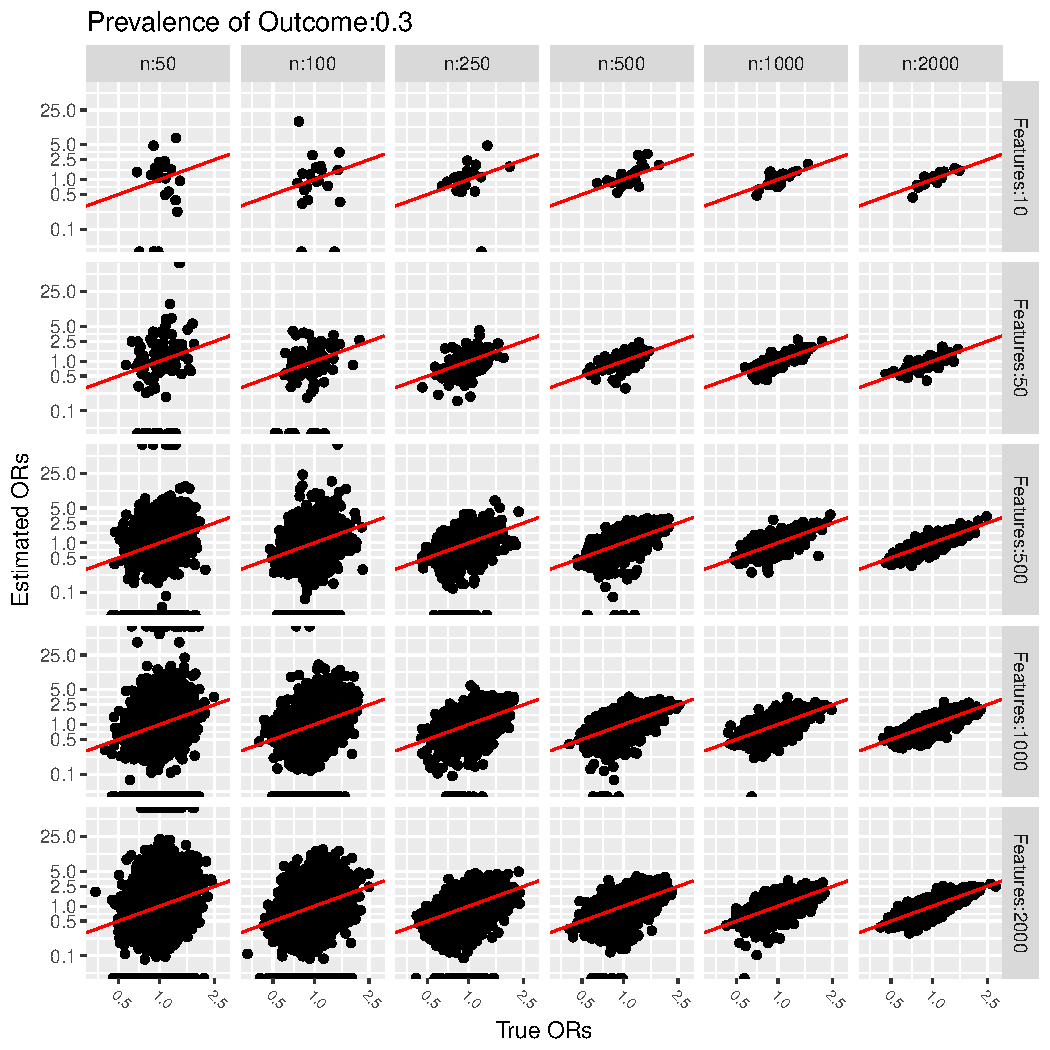
\includegraphics[width=\maxwidth]{hdata-simor-plotb-1} }

\end{Schunk}
The last two figures use a log scale for the $y$-axis (estimated odds
ratios), so the errors in estimating the odds ratios are quite
severe.  For a sample size of $n=50$ one cannot even estimate a single
pre-specified odds ratio.  To be able to accurately assess 10 ORs (10
candidate features) requires about $n=1000$.  To assess 2000 features,
a sample size of $n=2000$ seems adequate only for the very smallest
and very largest true ORs.

The plot below summarizes the previous plots by computing the 0.9 quantile of
the multiplicative margin of error (fold change) over the whole set of estimated
odds ratios, ignoring direction. 
\begin{Schunk}
\begin{Sinput}
ggplot(U, aes(x=n, y=mmoe)) + geom_point() + facet_grid(Features ~ Yprev) +
  geom_hline(aes(yintercept=1.5, col='red')) +
  ylim(1, 10) +
  ylab('0.9 Quantile of Multiplicative Margin of Error in OR Across Features')
\end{Sinput}


\centerline{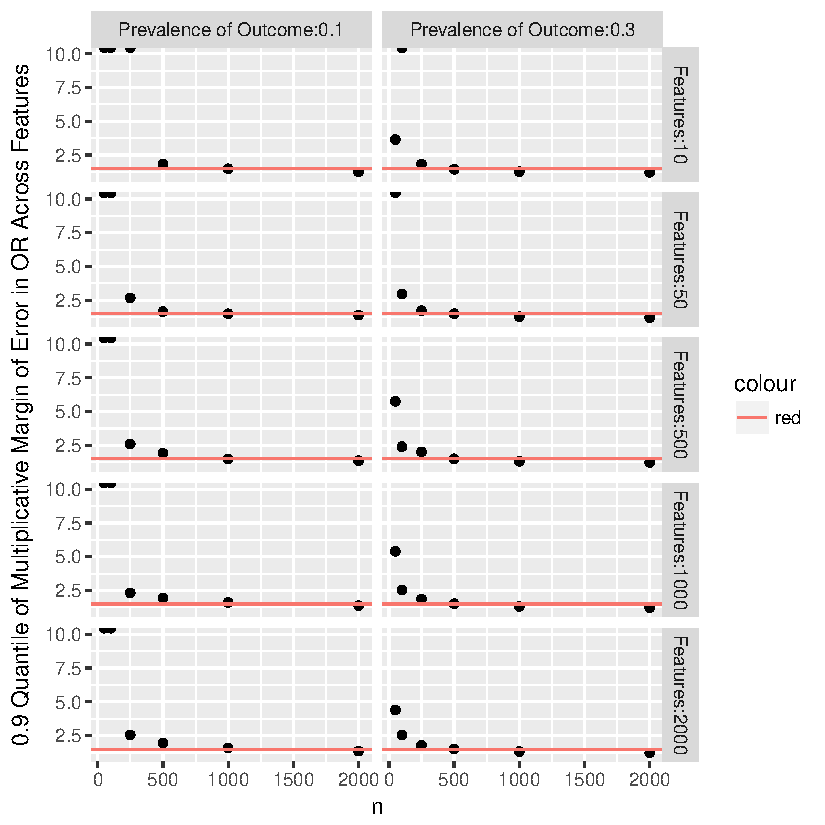
\includegraphics[width=\maxwidth]{hdata-simor-mmoe-1} }

\end{Schunk}
Horizontal red lines depict a multiplicative margin of error (MMOE) of
1.5 which may be considered the minimally acceptable error in
estimating odds ratios.  This was largely achieved with $n=1000$ for a
low-incidence $Y$, and $n=500$ for a moderate-incidence $Y$.

Another way to summarize the results is to compute the Spearman rank correlation
between estimated and true underlying odds ratios over the entire set of 
estimates.
\begin{Schunk}
\begin{Sinput}
ggplot(U, aes(x=n, y=rho)) + geom_point() +
  facet_grid(Features ~ Yprev) +
  ylab(expression(paste('Spearman ', rho, ' Rank Correlation Between ',
                        OR, ' and ', hat(OR), ' Across Features')))
\end{Sinput}


\centerline{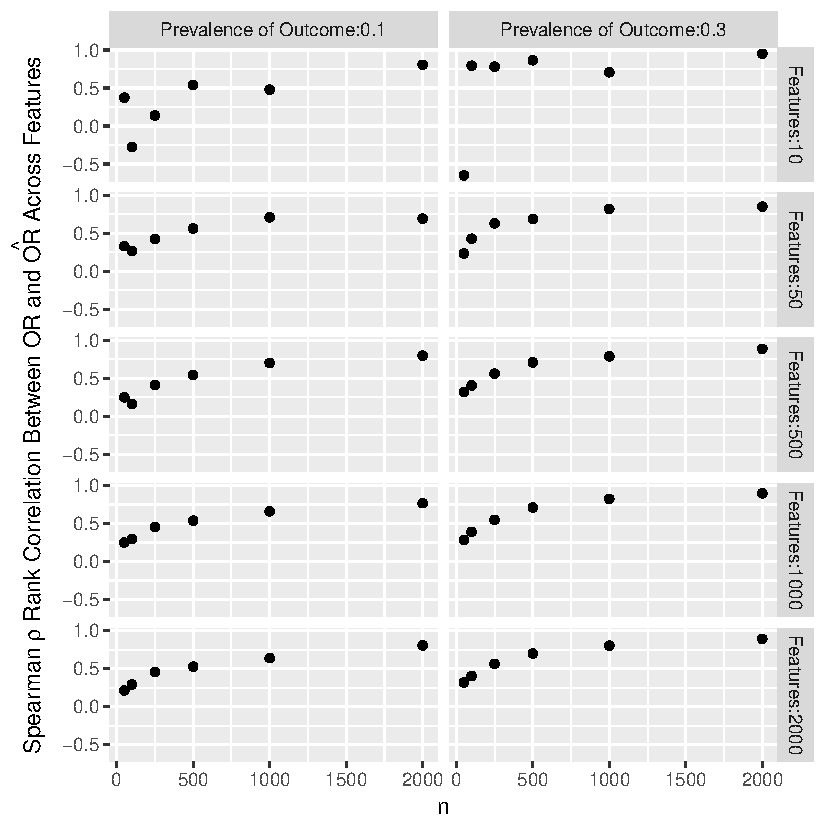
\includegraphics[width=\maxwidth]{hdata-simor-rho-1} }

\end{Schunk}
One may desire a correlation with the truth of say 0.8 and can solve
for the needed sample size.

\subsection{Bootstrap Analysis for One Simulated Dataset}
Suppose that one wanted to test $p$ candidate features and select the
most ``significant'' one for a validation study.  How likely is the
apparently ``best'' one to be truly the best?  What is a confidence
interval for the rank of this ``winner''?  How much bias in the OR
does the selection process create?  The bootstrap can be used to
answer all of these questions without needing to assume anything about
true population parameter values.  The bootstrap can take into account
many sources of uncertainty.  We use the bootstrap to estimate the
bias in the apparent highest and apparent lowest odds ratios---the two
``winners''.  The sample size of the simulated data is 600 subjects
and there are 300 candidate features.

The bootstrap is based on sampling with replacement from the rows of the entire 
data matrix $(X, Y)$.  In order to sample from the rows we need to generate raw 
data, not just numbers of ``successes'' and ``failures'' as in the last 
simulation.

\begin{Schunk}
\begin{Sinput}
# Function to simulate the raw data
# prev is the vector of prevalences of x when y=0 as before
# yprev is the overall prevalence of y
# n is the sample size
# or is the vector of true odds ratios
sim <- function(n, yprev, prev, or) {
  y <- rbinom(n, 1, yprev)
  p <- length(prev)
  if(p != length(or)) stop('prev and or must have the same length')

  # prev = Pr(x=1 | y=0); let the odds for this be oprev = prev / (1-prev)
  # or = odds(x=1 | y=1) / oprev
  # Pr(x=1 | y=1) = oprev / ((1 / or) + oprev)

  oprev <- prev / (1 - prev)
  p1 <- oprev / ((1 / or) + oprev)
  x <- matrix(NA, nrow=n, ncol=p)
  for(j in 1 : p) 
  	x[, j] <- ifelse(y == 1, rbinom(n, 1, prob = p1[j]  ), 
                             rbinom(n, 1, prob = prev[j]))
  list(x=x, y=y)
}
  
# Function to compute the sample odds ratios given x matrix and y vector
ors <- function(x, y) {
  p <- ncol(x)
  or <- numeric(p)
  for(j in 1 : p) {
    f <- table(x[, j], y)
    or[j] <- f[2, 2] * f[1, 1] / (f[1, 2] * f[2, 1])
  }
  or
}
\end{Sinput}
\end{Schunk}
      
\begin{Schunk}
\begin{Sinput}
# Generate sample of size 600 with 300 features
# Log odds ratios have a normal distribution with mean 0 SD 0.3
# x have a random prevalence uniform [0.05, 0.5]
# y has prevalence 0.3

set.seed(188)	
n <- 600; p <- 300
prev <- runif(p, .05, .5)
or   <- exp(rnorm(p, 0, .3))
z    <- sim(n, 0.3, prev, or)

# Compute estimated ORs
x <- z$x;   y <- z$y
sor <- ors(x, y)
# Show how estimates related to true ORs
ggplot(data.frame(or, sor), aes(x=or, y=sor)) + geom_point() +
  xlab('True OR') + ylab('Estimated OR')

# Print the largest estimated OR and its column number,
# and corresponding true OR, and similarly for the smallest.
largest   <- max(sor)
imax      <- which.max(sor)
true.imax <- or[imax]
mmoe.imax <- largest / true.imax
smallest  <- min(sor)
imin      <- which.min(sor)
true.imin <- or[imin]
mmoe.imin <- smallest / true.imin
cat('\nLargest observed OR\n')
\end{Sinput}
\begin{Soutput}

Largest observed OR
\end{Soutput}
\begin{Sinput}
cat('OR:', round(largest, 2), '  Feature #', imax, '  True OR:',
    round(true.imax, 2), '  MMOE:', round(mmoe.imax, 2), '\n')
\end{Sinput}
\begin{Soutput}
OR: 2.94   Feature # 90   True OR: 1.71   MMOE: 1.72 
\end{Soutput}
\begin{Sinput}
cat('Rank of winning feature among true ORs:', sum(or <= or[imax]), '\n\n')
\end{Sinput}
\begin{Soutput}
Rank of winning feature among true ORs: 285 
\end{Soutput}
\begin{Sinput}
cat('Smallest observed OR\n')
\end{Sinput}
\begin{Soutput}
Smallest observed OR
\end{Soutput}
\begin{Sinput}
cat('OR:', round(smallest, 2), '  Feature #', imin, '  True OR:',
    round(true.imin, 2), '  MMOE:', round(mmoe.imin, 2), '\n')
\end{Sinput}
\begin{Soutput}
OR: 0.21   Feature # 99   True OR: 0.71   MMOE: 0.3 
\end{Soutput}


\centerline{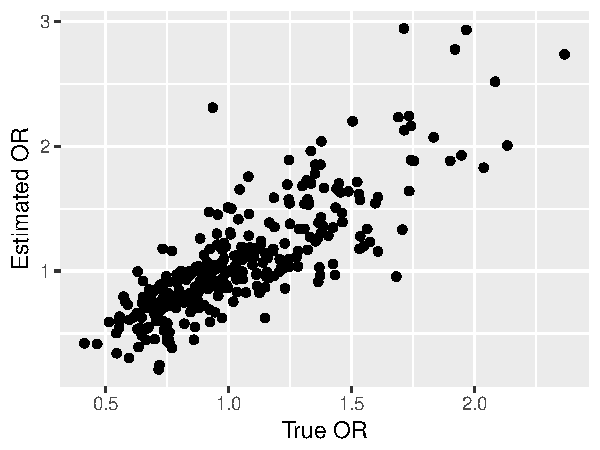
\includegraphics[width=\maxwidth]{hdata-simbd-1} }

\end{Schunk}

Next use the bootstrap to get an estimate of the MMOE for the observed
largest OR, and a 0.95 confidence 
interval for the true unknown rank of the largest observed OR from
among all the features.  1000 bootstrap resamples are drawn.  In
estimating the MMOE we are estimating bias in the largest log odds
ratio when a new ``largest'' OR is found in each bootstrap resample.
That estimated OR is compared to the OR evaluated in the whole sample
for the same column number.  This is also done for the ``smallest'' OR.

\begin{Schunk}
\begin{Sinput}
set.seed(11)
B <- 1000
ranksS <- ranksL <- mmoeS <- mmoeL <- numeric(B)

for(k in 1 : B) {
  # Draw a sample of size n with replacement
  i <- sample(1 : n, n, replace=TRUE)
  # Compute sample ORs on the new sample
  bor      <- ors(x[i, ], y[i])
  blargest <- max(bor)
  bmax     <- which.max(bor)
  ranksL[k] <- sum(bor <= largest)
  mmoeL[k]  <- blargest / sor[bmax]
  bsmallest <- min(bor)
  bmin      <- which.min(bor)
  ranksS[k] <- sum(bor <= smallest)
  mmoeS[k]  <- bsmallest / sor[bmin]
}
\end{Sinput}
\end{Schunk}

The bootstrap geometric mean MMOE for the smallest odds ratio was zero
due to small frequencies in some $X$s.  The median bootstrap MMOE was
used to bias-correct the observed smallest OR, while the geometric
mean was used for the largest.
\begin{Schunk}
\begin{Sinput}
pr <- function(which, ranks, mmoe, mmoe.true, estor, or.true) {
  gm <- exp(mean(log(mmoe)))
  cat(which, 'OR\n')
  cat('CL for rank:', quantile(ranks, c(0.025, 0.975)),
      '  Median MMOE:', round(median(mmoe), 2),
      '  Geometric mean MMOE:', round(gm, 2),
      '\nTrue MMOE:', round(mmoe.true, 2), '\n')
  bmmoe <- if(which == 'Largest') gm else median(mmoe)
  cat('Bootstrap bias-corrected', tolower(which), 'OR:',
      round(estor / bmmoe, 2),
      '  Original OR:', round(estor, 2),
      '  True OR:', round(or.true, 2),
      '\n\n')
}
pr('Largest',  ranksL, mmoeL, mmoe.imax, largest,  true.imax)
\end{Sinput}
\begin{Soutput}
Largest OR
CL for rank: 294 299   Median MMOE: 1.45   Geometric mean MMOE: 1.52 
True MMOE: 1.72 
Bootstrap bias-corrected largest OR: 1.94   Original OR: 2.94   True OR: 1.71 
\end{Soutput}
\begin{Sinput}
pr('Smallest', ranksS, mmoeS, mmoe.imin, smallest, true.imin)
\end{Sinput}
\begin{Soutput}
Smallest OR
CL for rank: 0 5   Median MMOE: 0.32   Geometric mean MMOE: 0 
True MMOE: 0.3 
Bootstrap bias-corrected smallest OR: 0.67   Original OR: 0.21   True OR: 0.71 
\end{Soutput}
\end{Schunk}

The bootstrap bias-corrected ORs took the observed extreme ORs and
multiplied them by their respective bootstrap geometric mean or median
MMOEs.  The bias-corrected estimates are closer to the true ORs.

The data are consistent with the observed smallest OR truly being in the
bottom 5 and the observed largest OR truly being in the top 7.

Here is some example wording that could be used in a statistical
analysis plan: We did not evaluate the probability that non-selected genes
are truly unimportant but will accompany the planned gene screening
results with a bootstrap analysis to compute 0.95 confidence intervals
for the rank of each gene, using a non-directional measure of
association when ranking.  The ``winning'' genes will have high ranks in
competing with each other (by definition) but if the lower confidence
limits include mid- to low-level ranks the uncertainty of these
winners will be noted.  Conversely, if the upper confidence intervals
of ranks of ``losers'' extend well into the ranks of ``winners'', the
uncertainty associated with our ability to rule out ``losers'' for
further investigation will be noted. 
